%% LLT: Turn off some annoying warnings...
\RequirePackage{silence}
\WarningFilter{titlesec}{Non standard sectioning command}
\WarningFilter{scrreprt}{Usage of package}
\WarningFilter{scrreprt}{Activating an ugly workaround}

% **************************************************
% Document Class Definition
% **************************************************
\documentclass[%
	paper=A4,					% paper size --> A4 is default in Germany
%	twoside=true,				% onesite or twoside printing
    oneside=true,
%	twoside=false,				% onesite or twoside printing
	openright,					% doublepage cleaning ends up right side
	parskip=full,				% spacing value / method for paragraphs
	chapterprefix=true,			% prefix for chapter marks
	11pt,						% font size
	headings=normal,			% size of headings
	bibliography=totoc,			% include bib in toc
	listof=totoc,				% include listof entries in toc
	titlepage=on,				% own page for each title page
	captions=tableabove,		% display table captions above the float env
	draft=false,				% value for draft version
]{scrreprt}%

\usepackage[utf8]{inputenc}		% defines file's character encoding
\usepackage{paralist}          % for compactitem itemization

% **************************************************
% Debug LaTeX Information
% **************************************************
%\listfiles

% **************************************************
% Information and Commands for Reuse
% **************************************************
\newcommand{\thesisTitle}{Praxisbericht}
\newcommand{\thesisName}{Tom Oberhauser}
\newcommand{\thesisSubject}{12 wöchiges Praktikum beim Deutschen Forschungszentrum für Künstliche Intelligenz}
\newcommand{\thesisDate}{August 26, 2015}
%\newcommand{\thesisVersion}{Final}

\newcommand{\thesisFirstReviewer}{Prof. Christoph Knabe}
\newcommand{\thesisFirstReviewerUniversity}{\protect{Beuth Hochschule für Technik Berlin}}
\newcommand{\thesisFirstReviewerDepartment}{Fachbereich VI - Informatik und Medien}

\newcommand{\thesisSecondReviewer}{Dr. Philippe Thomas}
\newcommand{\thesisSecondReviewerUniversity}{\protect{Deutsches Forschungszentrum für Künstliche Intelligenz}}
\newcommand{\thesisSecondReviewerDepartment}{Forschungsgruppe Sprachtechnologie (DFKI-LT)}

%\newcommand{\thesisFirstSupervisor}{Jane Doe}
%\newcommand{\thesisSecondSupervisor}{John Smith}

\newcommand{\thesisUniversity}{\protect{12 wöchiges Praktikum beim Deutschen Forschungszentrum für Künstliche Intelligenz}}
\newcommand{\thesisUniversityDepartment}{Forschungsgruppe Sprachtechnologien (DFKI-LT)}
\newcommand{\thesisUniversityInstitute}{Projekt ``Smart Data for Mobility'' (SD4M)}
%\newcommand{\thesisUniversityGroup}{Clean Thesis Group (CTG)}
\newcommand{\thesisUniversityCity}{Berlin}
%\newcommand{\thesisUniversityStreetAddress}{Street address}
%\newcommand{\thesisUniversityPostalCode}{Postal Code}

% **************************************************
% Load and Configure Packages
% **************************************************

\usepackage[ngerman]{babel} % babel system, adjust the language of the content
\usepackage[					% clean thesis style
	figuresep=colon,%
	sansserif=false,%
	hangfigurecaption=false,%
	hangsection=true,%
	hangsubsection=true,%
	colorize=full,%
	colortheme=bluemagenta,%
% LLT: Use biber if using UTF8 encoding
% 	bibsys=bibtex,%
	bibsys=biber,%
	bibfile=bib-refs,%
	bibstyle=alphabetic,%
]{cleanthesis}

\hypersetup{					% setup the hyperref-package options
	pdftitle={\thesisTitle},	% 	- title (PDF meta)
	pdfsubject={\thesisSubject},% 	- subject (PDF meta)
	pdfauthor={\thesisName},	% 	- author (PDF meta)
	plainpages=false,			% 	-
	colorlinks=false,			% 	- colorize links?
	pdfborder={0 0 0},			% 	-
	breaklinks=true,			% 	- allow line break inside links
	bookmarksnumbered=true,		%
	bookmarksopen=true			%
}

% **************************************************
% Document CONTENT
% **************************************************
\begin{document}

% --------------------------
% rename document parts
% --------------------------
\renewcaptionname{ngerman}{\figurename}{Abb.}
\renewcaptionname{ngerman}{\tablename}{Tab.}
%\renewcaptionname{english}{\figurename}{Fig.}
%\renewcaptionname{english}{\tablename}{Tab.}

% --------------------------
% Front matter
% --------------------------
\pagenumbering{roman}			% roman page numbing (invisible for empty page style)
\pagestyle{empty}				% no header or footers
% !TEX root = ../thesis-example.tex
%
% ------------------------------------  --> cover title page
%\begin{titlepage}
%	\pdfbookmark[0]{Cover}{Cover}
%	\flushright
%	\hfill
%	\vfill
%	{\LARGE\thesisTitle \par}
%	\rule[5pt]{\textwidth}{.4pt} \par
%	{\Large\thesisName}
%	\vfill
%	\textit{\large\thesisDate} \\
%	Version: \thesisVersion
%\end{titlepage}


% ------------------------------------  --> main title page
\begin{titlepage}
	\pdfbookmark[0]{Titlepage}{Titlepage}
	\tgherosfont
	\centering

	{\Large \thesisUniversity} \\[4mm]
	
\includegraphics[width=6cm]{gfx/Clean-Thesis-Logo} \\[2mm]
	\textsf{\thesisUniversityDepartment} \\
	\textsf{\thesisUniversityInstitute} \\
	\textsf{\thesisUniversityGroup} \\

	\vfill
	{\large \thesisSubject} \\[5mm]
	{\LARGE \color{ctcolortitle}\textbf{\thesisTitle} \\[10mm]}
	{\Large \thesisName} \\

	\vfill
	\begin{minipage}[t]{.27\textwidth}
		\raggedleft
		\textit{1. Reviewer}
	\end{minipage}
	\hspace*{15pt}
	\begin{minipage}[t]{.65\textwidth}
		{\Large \thesisFirstReviewer} \\
	  	{\small \thesisFirstReviewerDepartment} \\[-1mm]
		{\small \thesisFirstReviewerUniversity}
	\end{minipage} \\[5mm]
	\begin{minipage}[t]{.27\textwidth}
		\raggedleft
		\textit{2. Reviewer}
	\end{minipage}
	\hspace*{15pt}
	\begin{minipage}[t]{.65\textwidth}
		{\Large \thesisSecondReviewer} \\
	  	{\small \thesisSecondReviewerDepartment} \\[-1mm]
		{\small \thesisSecondReviewerUniversity}
	\end{minipage} \\[10mm]
	\begin{minipage}[t]{.27\textwidth}
		\raggedleft
		\textit{Supervisors}
	\end{minipage}
	\hspace*{15pt}
	\begin{minipage}[t]{.65\textwidth}
		\thesisFirstSupervisor\ and \thesisSecondSupervisor
	\end{minipage} \\[10mm]

	\thesisDate \\

\end{titlepage}


% ------------------------------------  --> lower title back for single page layout
%\hfill
%\vfill
%{
%	\small
%	\textbf{\thesisName} \\
%	\textit{\thesisTitle} \\
%	\thesisSubject, \thesisDate \\
%	Reviewers: \thesisFirstReviewer\ and \thesisSecondReviewer \\
%	Supervisors: \thesisFirstSupervisor\ and \thesisSecondSupervisor \\[1.5em]
%	\textbf{\thesisUniversity} \\
%	\textit{\thesisUniversityGroup} \\
%	\thesisUniversityInstitute \\
%	\thesisUniversityDepartment \\
%	\thesisUniversityStreetAddress \\
%	\thesisUniversityPostalCode\ and \thesisUniversityCity
%}
		% INCLUDE: all titlepages
\cleardoublepage

\setcounter{tocdepth}{2}		% define depth of toc
\tableofcontents				% display table of contents
\cleardoublepage

% --------------------------
% Body matter
% --------------------------
\pagenumbering{arabic}			% arabic page numbering
\setcounter{page}{1}			% set page counter
\pagestyle{maincontentstyle} 	% fancy header and footer

\chapter{Einleitung}
\label{sec:intro}
\section{Vorstellung des Praktikumsbetriebes}
\label{sec:intro:dfki}
Das Deutsche Forschungszentrum für Künstliche Intelligenz GmbH, im folgenden DFKI genannt, wurde 1988 gegründet.
Es unterhält Standorte in Kaiserslautern, Saarbrücken, Bremen und ein Projektbüro in Berlin.
Mit seinen 478 Mitarbeiten sowie 337 studentischen Mitarbeiten erforscht und entwickelt das DFKI innovative Softwaretechnologien auf der Basis von Methoden der Künstlichen Intelligenz.
Die notwendigen Gelder werden durch Ausschreibungen öffentlicher Fördermittelgeber wie der Europäischen Union, dem Bundesministerium für Bildung und Forschung (BMBF), dem Bundesministerium für Wirtschaft und Technologie (BMWi), den Bundesländern und der Deutschen Forschungsgemeinschaft (DFG) sowie durch Entwicklungsaufträge aus der Industrie akquiriert.\footnote{http://www.dfki.de/web/ueber}
\\\\
Ich absolvierte mein Praktikum innerhalb der \textit{Forschungsgruppe Sprachtechnologie}, einer von 15 Forschungsgruppen\footnote{http://www.dfki.de/web/ueber/orgaeinheiten} des DFKI, im Projektbüro Berlin. Die Gruppe wird geleitet durch Prof. Dr. Hans Uszkoreit.\footnote{http://www.dfki.de/lt/}.
\\\\
Meine Aufgabengebiete konzentrierten sich um das Projekt \textit{''SD4M - Smart Data for Mobility''}. Das DFKI ist hier Teil eines Konsortiums aus 5 Partnern unter der Konsortialführung der \textit{DB Systel GmbH}.\footnote{http://sd4m.net/#konsortium}. 
Das Projekt \textit{SD4M} wird in Abschnitt \ref{sec:main:overview:sd4m} auf Seite \pageref{sec:main:overview:sd4m} näher erläutert.
\section{Weg zur Praktikumsstelle}
\label{sec:intro:wegZurPraktikumsstelle}
Herr Prof. Dr. habil. Alexander Löser aus dem Fachbereich VI der Beuth Hochschule für Technik Berlin machte mich auf den Praktikumsplatz aufmerksam. Durch seine Mitarbeit in Projekten im DFKI Projektbüro Berlin hatte er mitbekommen, dass Bedarf und Interesse an Praktikanten und studentischen Mitarbeitern besteht und mich angeschrieben. Nach einem persönlichen Gespräch mit dem Leiter der Forschungsgruppe, Prof. Dr. Hans Uszkoreit, kam es zur Vertragsunterzeichnung.
\chapter{Tätigkeitsbereiche und Aufgaben}
\section{Überblick}
SD4M erklären.. erklären warum die Daten aufbereitet werden mussten
\section{Vorbereitung der Arbeitsumgebung}
Eigener Rechner, lokale Umgebung, DB ... warum?
\section{Einarbeitung}
\section{Aufgaben}
\subsection{Extraktion einer Straßenliste}
\subsection{Verknüpfung von Daten der Deutschen Bahn mit Daten aus OpenStreetMap}
\subsection{Datenaufwertung??}

\chapter{Fazit}
\section{Praktikum und Studium}
\section{Bewertung des Praktikums}

\appendix
\chapter{Anlagen}
\section{Well-Known-Binary Format (WKB)}
\label{sec:appendix:wkb}
Das \textit{Well-Known-Binary} Format ist die binäre Repräsentation eines geometrischen Objekts des \textit{Simple Feature Models}.
Das Simple Feature Model ist eine Untermenge des ISO 19107 Standards, welcher die geometrischen Eigenschaften von Geoobjekten spezifiziert. Ausgehend von einer allgemeinen Oberklasse können geometrische Primitive, wie z.B. ein Punkt, oder komplexe geometrische Objekte, wie z.B. Flächen oder Sammlungen von Objekten, beschrieben werden. (vgl. \cite{Bill2010}:358ff.). Die verfügbaren Klassen werden in Abbildung \ref{fig:bill_sfm} aufgezeigt.
\begin{figure}[!htb]
  \centering
   \fbox{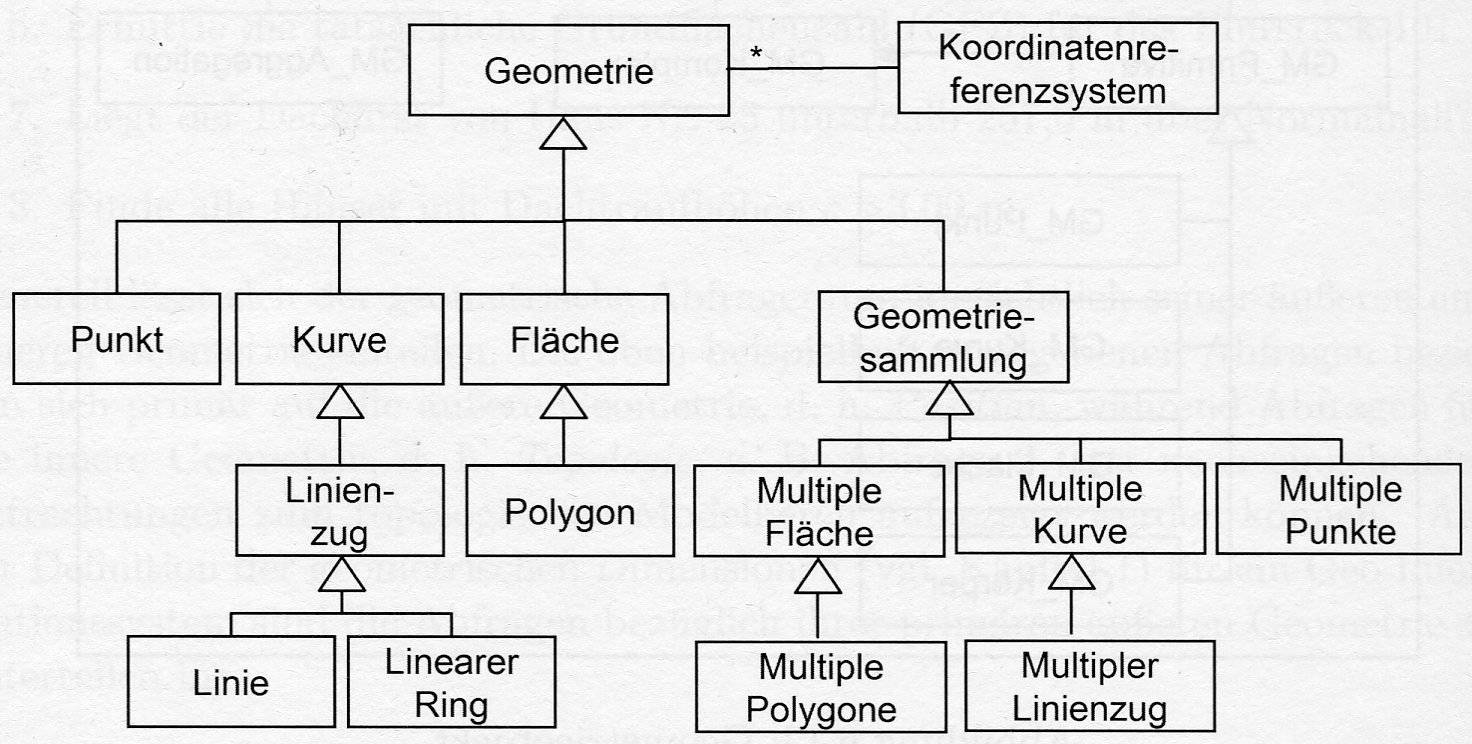
\includegraphics[width=1\textwidth]{gfx/bill_sfm001.jpg}}
   \caption{Geometrien im Simple Feature Model \protect\cite{Bill2010}:360}
   \label{fig:bill_sfm}
\end{figure}

Das WKB Format wird beispielsweise innerhalb der PostgreSQL Erweiterung PostGIS\footnote{http://postgis.net} genutzt, um geometrische Objekte in einer Datenbank abzulegen.
Analog dazu existiert das \textit{Well-Known-Text} Format, welches die textuelle Repräsentation geometrische Objekte des Simple Feature Models spezifiziert.

\subsubsection{Beispiel für das WKB und das WKT Format}
Ein Punkt mit den Koordinaten \texttt{13.439561 Ost} sowie \texttt{52.54002 Nord} entspricht der WKT Repräsentation\\\\
\texttt{SRID=4326;POINT(13.439561 52.54002)}\\\\
und der WKB Repräsentation\\\\
\texttt{0101000020E6100000B131AF230EE12A40CC9717601F454A40}\\\\
Der Wert \texttt{SRID} beinhaltet die ID des zu verwendenden Koordinatenreferenzsystems.
Die ID \texttt{4326} entspricht dem häufig verwendeten Referenzsystem \texttt{WGS84}\footnote{http://spatialreference.org/ref/epsg/4326/}.  

\section{GeoJSON}
\label{sec:appendix:geojson}
GeoJSON\footnote{http://geojson.org} ist ein Format zur Repräsentation von geometrischen Objekten im JSON Format.
Es verwendet ein ähnliches hierarchisches Klassenmodell. (vgl. \cite{WEB:GEOJSON:Spec:2008}).

\subsubsection{Beispiel für das GeoJSON Format}
Ein Punkt mit den Koordinaten \texttt{13.439561 Ost} sowie \texttt{52.54002 Nord} entspricht der GeoJSON Repräsentation
\lstset{
  numbers=none,
  caption=Beispiel eines geometrischen Punktes in GeoJSON Repräsentation,
  label=
}
\begin{lstlisting}
  {
    "type": "Point",
    "coordinates": [
        13.439561,
        52.54002
    ]
}
\end{lstlisting}

\section{OpenStreetMap Datenformat}
\label{sec:appendix:osm:data}
OpenStreetMap bietet seine Daten zum Download in einer Datei, \textit{planet.osm}\footnote{http://planet.openstreetmap.org/}, an. Diese Datei im XML-Format enthält den kompletten Datenbestand des OpenStreetMap Projekts. 
Da diese Datei sehr groß ist (gepackt ca. 50GB) bieten andere Dienstleister wie zum Beispiel die Geofabrik GmbH Karlsruhe\footnote{http://www.geofabrik.de} auch kleinere Bereiche des Datenbestandes, zum Beispiel nur Deutschland, an.
Zur Speicherung der Daten werden die Elemente \textit{Nodes}, \textit{Ways} und \textit{Relations} verwendet. (vgl. \cite{WEB:OSM:Primitives:2015})
\begin{compactitem}
  \item \textbf{Nodes}, ein geometrischer Punkt, welcher durch geographische Breite und Länge bestimmt ist
  \item \textbf{Ways}, ein Linienzug zwischen mehreren Punkten. Hiermit werden zum Beispiel Straßen, Flüsse und vieles mehr modelliert
  \item \textbf{Relations}, eine logische Gruppierung mehrerer \textit{Nodes}, \textit{Ways} oder auch \textit{Relations}. Die Mitglieder einer Relation haben einen Bezug zueinander, zum Beispiel ein Wald mit seinen Lichtungen oder ein Bahnhof. 
\end{compactitem}
Die Bedeutung der Elemente wird durch Key-Value Paare, sogenannte \textit{Tags}, beschrieben. Hier wird beispielsweise festgelegt, ob ein Way eine Straße abbildet oder einen Fluss.

\subsubsection{Beispiel eines Nodes}

\lstset{
  numbers=none,
  caption=Beispiel eines Nodes aus planet.osm,
  label=
}
\begin{lstlisting}
<node id="3637807236" visible="true" version="1" changeset="32456135" timestamp="2015-07-06T19:04:03Z" user="bigbug21" uid="15748" lat="50.5379840" lon="12.1402231"/>
\end{lstlisting}

\subsubsection{Beispiel eines Ways}
\lstset{
  numbers=none,
  caption=Beispiel eines Ways aus planet.osm,
  label=
}
\begin{lstlisting}
  <way id="358952758" visible="true" version="1" changeset="32456135" timestamp="2015-07-06T19:04:13Z" user="bigbug21"  uid="15748">
  <nd ref="3637807236"/>
  <nd ref="3637807232"/>
  <nd ref="3637807230"/>
  <nd ref="3637806843"/>
  <nd ref="3637806841"/>
  <tag k="public_transport" v="platform"/>
  <tag k="railway" v="platform"/>
  <tag k="train" v="yes"/>
 </way>
\end{lstlisting}

\subsubsection{Beispiel einer Relation}
\lstset{
  numbers=none,
  caption=Beispiel einer Relation aus planet.osm
}
\begin{lstlisting}
<relation id="2303826" visible="true" version="9" changeset="34783224" timestamp="2015-10-21T17:05:38Z" user="Kakaner" uid="1851521">
  <member type="way" ref="166800600" role=""/>
  <member type="way" ref="166800590" role=""/>
  <member type="way" ref="166800593" role=""/>
  <member type="way" ref="166800357" role=""/>
  <member type="way" ref="376274301" role=""/>
  <member type="way" ref="166800198" role=""/>
  <member type="way" ref="165821978" role=""/>
  <member type="way" ref="165821752" role=""/>
  <member type="way" ref="165741930" role=""/>
  <member type="way" ref="165741583" role=""/>
  <member type="way" ref="165479804" role=""/>
  <member type="way" ref="165479800" role=""/>
  <member type="way" ref="165479712" role=""/>
  <member type="way" ref="165409360" role=""/>
  <member type="way" ref="165408947" role=""/>
  <member type="way" ref="264419428" role=""/>
  <member type="way" ref="165022595" role=""/>
  <member type="way" ref="165022069" role=""/>
  <member type="way" ref="164988309" role=""/>
  <member type="way" ref="164987948" role=""/>
  <member type="way" ref="159213270" role=""/>
  <member type="way" ref="264419420" role=""/>
  <member type="way" ref="376165609" role=""/>
  <member type="way" ref="158208266" role=""/>
  <member type="way" ref="159211943" role=""/>
  <member type="way" ref="264419427" role=""/>
  <member type="way" ref="356950454" role=""/>
  <member type="way" ref="158207942" role=""/>
  <member type="way" ref="158206932" role=""/>
  <member type="way" ref="250106659" role=""/>
  <member type="way" ref="250106648" role=""/>
  <member type="way" ref="254270906" role=""/>
  <member type="way" ref="158511899" role=""/>
  <member type="way" ref="158511802" role=""/>
  <member type="way" ref="159211993" role=""/>
  <tag k="operator" v="Vogtlandbahn"/>
  <tag k="public_transport:version" v="2"/>
  <tag k="ref" v="VB2"/>
  <tag k="route" v="train"/>
  <tag k="type" v="route"/>
 </relation>
\end{lstlisting}

\section{Beispiel einer Straße in OpenStreetMap}
\label{sec:appenix:osm:streets}
Im folgenden Abschnitt soll am Beispiel eines Teilabschnittes einer Straße (siehe Abbildung \ref{fig:osm_streets_1}) gezeigt werden, in welcher Form Straßen innerhalb der OpenStreetMap Daten vorliegen.
Eine Straße ist entweder ein einzelner, oder eine Verkettung aus \textit{Ways} mit gesetztem \texttt{highway} Tag.
Im Listing \ref{code:osm_streets} Zeile 13 und 44 ist ein Beispiel dafür ersichtlich. Beispielsweise bedeutet der Wert \texttt{''primary''} Bundesstraße oder \texttt{''motorway''} Autobahn.
\begin{figure}[htb]
  \centering
   \fbox{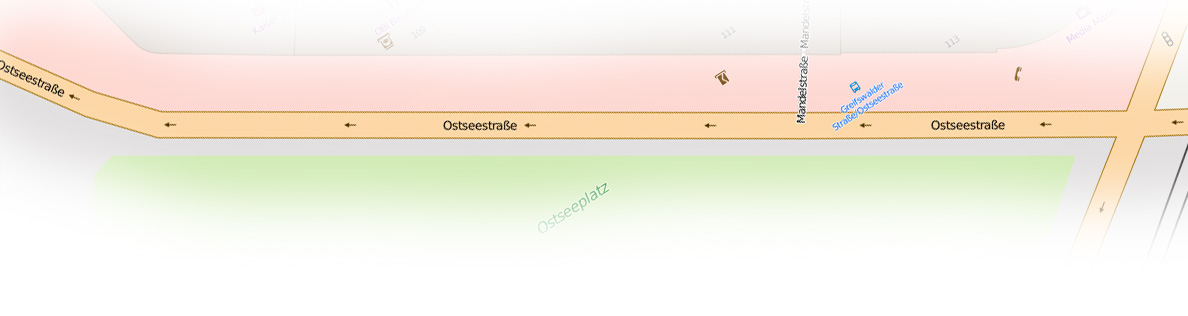
\includegraphics[width=1\textwidth]{gfx/osm_streets_1.jpg}}
   \caption{Teilausschnitt der Greifswalder Straße}
   \label{fig:osm_streets_1}
\end{figure}
Die Unterteilung einer Straße in mehrere Ways ist mitunter notwendig, da an einem Way-Element alle Daten des aktuellen Straßenabschnitts, wie z.B. die zulässige Höchstgeschwindigkeit, durch \textit{Tags} gespeichert sind. Sofern sich diese Daten im Straßenverlauf ändern, wird dies durch einen separates Way-Element wiedergegeben.
Der hier gezeigte Teilabschnitt ist ebenfalls bereits in zwei separate Way-Elemente mit den ID´s \texttt{241186022} und \texttt{4615358} untergliedert (Abbildung \ref{fig:osm_streets_2}).
\begin{figure}[htb]
  \centering
   \fbox{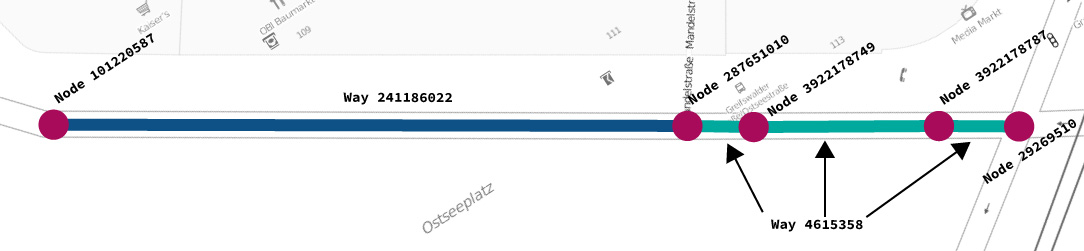
\includegraphics[width=1\textwidth]{gfx/osm_streets_2.jpg}}
   \caption{Beispiel für multiple Ways einer Straße}
   \label{fig:osm_streets_2}
\end{figure}
Dies war notwendig, da sich die Anzahl der Fahrspuren geändert hat.
Der Tag mit dem Key ``lanes'' hat seinen Wert von \texttt{2} auf \texttt{3} geändert. Die Änderung ist im Listing \ref{code:osm_streets} auf Zeile 28 und 45 ersichtlich.
\lstset{
  numbers=left,
  numbersep=5pt,
  caption=Vollständige Daten des Straßenabschnitts,
  label=code:osm_streets
}
\begin{lstlisting}
<node id="101220587" visible="true" version="11" changeset="18256244" timestamp="2013-10-08T22:00:56Z" user="Peter Maiwald" uid="90528" lat="52.5464853" lon="13.4424534"/>
<node id="287651010" visible="true" version="5" changeset="23075493" timestamp="2014-06-22T09:26:32Z" user="atpl_pilot" uid="881429" lat="52.5459138" lon="13.4438910"/>
<node id="3922178749" visible="true" version="1" changeset="36300926" timestamp="2016-01-01T16:28:14Z" user="Balgofil" uid="95702" lat="52.5458508" lon="13.4440518">
 <tag k="bus" v="yes"/>
 <tag k="name" v="Greifswalder Straße/Ostseestraße"/>
 <tag k="public_transport" v="stop_position"/>
 <tag k="ref:BVG" v="105416"/>
 <tag k="website" v="http://qr.bvg.de/h105416"/>
 <tag k="wheelchair" v="limited"/>
</node>
<node id="3922178787" visible="true" version="1" changeset="36300926" timestamp="2016-01-01T16:28:15Z" user="Balgofil" uid="95702" lat="52.5456743" lon="13.4445025">
 <tag k="crossing" v="traffic_signals"/>
 <tag k="highway" v="crossing"/>
</node>
<node id="29269510" visible="true" version="11" changeset="36300926" timestamp="2016-01-01T16:28:39Z" user="Balgofil" uid="95702" lat="52.5456175" lon="13.4446475">
 <tag k="TMC:cid_58:tabcd_1:Class" v="Point"/>
 <tag k="TMC:cid_58:tabcd_1:Direction" v="negative"/>
 <tag k="TMC:cid_58:tabcd_1:LCLversion" v="9.00"/>
 <tag k="TMC:cid_58:tabcd_1:LocationCode" v="21554"/>
 <tag k="TMC:cid_58:tabcd_1:NextLocationCode" v="21555"/>
 <tag k="TMC:cid_58:tabcd_1:PrevLocationCode" v="21553"/>
</node>
<way id="241186022" visible="true" version="4" changeset="35323067" timestamp="2015-11-15T08:45:00Z" user="anbr" uid="43566">
 <nd ref="287651010"/>
 <nd ref="101220587"/>
 <tag k="cycleway" v="lane"/>
 <tag k="highway" v="primary"/>
 <tag k="lanes" v="3"/>
 <tag k="maxspeed" v="50"/>
 <tag k="name" v="Ostseestraße"/>
 <tag k="oneway" v="yes"/>
 <tag k="postal_code" v="10409"/>
 <tag k="ref" v="L 1004"/>
 <tag k="sidewalk" v="right"/>
 <tag k="turn:lanes" v="left|none|none"/>
 <tag k="wikipedia" v="de:Ostseestraße"/>
</way>
<way id="4615358" visible="true" version="27" changeset="36300926" timestamp="2016-01-01T16:28:33Z" user="Balgofil" uid="95702">
 <nd ref="29269510"/>
 <nd ref="3922178787"/>
 <nd ref="3922178749"/>
 <nd ref="287651010"/>
 <tag k="cycleway" v="lane"/>
 <tag k="highway" v="primary"/>
 <tag k="lanes" v="2"/>
 <tag k="maxspeed" v="50"/>
 <tag k="name" v="Ostseestraße"/>
 <tag k="oneway" v="yes"/>
 <tag k="postal_code" v="10409"/>
 <tag k="ref" v="L 1004"/>
 <tag k="sidewalk" v="right"/>
 <tag k="wikipedia" v="de:Ostseestraße"/>
</way>
\end{lstlisting}
\lstset{
  numbers=none,
  caption=,
  label=
  }

\section{Beispiel zur Verwendung von JGraphT zur Trennung eines Graphen in zusammenhängende Elemente}
\label{sec:appendix:jgrapht_separation}
\lstset{
  language=Java,
  numbers=left,
  caption=Beispiel der Trennung eines Graphen in verbundene Teile,
  label=jgrapht_separation,
  keywordstyle=\color{javapurple}\bfseries,
  stringstyle=\color{javared},
  commentstyle=\color{javagreen},
  morecomment=[s][\color{javadocblue}]{/**}{*/},
}
\begin{lstlisting}
import org.jgrapht.UndirectedGraph;
import org.jgrapht.alg.ConnectivityInspector;
import org.jgrapht.graph.DefaultEdge;
import org.jgrapht.graph.SimpleGraph;

// ...
 
// Lege neuen leeren Graphen an, Knoten sind Objekte vom Typ Long
UndirectedGraph<Long, DefaultEdge> graph = new SimpleGraph<>(DefaultEdge.class);
// Graph mit 4 Knoten und 2 Kanten befüllen
Long v1 = new Long(1);
Long v2 = new Long(2);
Long v3 = new Long(3);
Long v4 = new Long(4);
graph.addVertex(v1);
graph.addVertex(v2);
graph.addVertex(v3);
graph.addVertex(v4);
graph.addEdge(v1, v2);
graph.addEge(v3, v4);
// Erzeuge neuen ConnectivityInspector
ConnectivityInspector<Long, DefaultEdge> ci = new ConnectivityInspector<>(graph);
// Erzeuge eine Liste von Sets mit zusammenhängenden Knoten
// Hier werden jetzt zwei Sets erzeugt. (1,2) und (3,4)
List<Set<Long>> connectedNodes = ci.connectedSets(); 
\end{lstlisting}
  
\section{GraphSeparator.java}
\label{sec:appenix:ose:graphseparator}
\lstset{
  language=Java,
  numbers=left,
  label=,
  caption=GraphSeparator.java,
  keywordstyle=\color{javapurple}\bfseries,
  stringstyle=\color{javared},
  commentstyle=\color{javagreen},
  morecomment=[s][\color{javadocblue}]{/**}{*/},
}
\begin{lstlisting}
package de.dfki.OsmosisStreetExtractor.util.geo;

import de.dfki.OsmosisStreetExtractor.util.database.OsmosisDB;
import de.dfki.OsmosisStreetExtractor.util.database.StreetGroup;
import org.jgrapht.UndirectedGraph;
import org.jgrapht.alg.ConnectivityInspector;
import org.jgrapht.graph.DefaultEdge;
import org.jgrapht.graph.SimpleGraph;

import java.util.ArrayList;
import java.util.HashMap;
import java.util.List;
import java.util.Set;

/**
* Created by Tom Oberhauser
* This class is used to separate a whole wayset (i.e. streets) into separate parts
*/
public class GraphSeparator {
  
  private final ArrayList<ArrayList<Long>> clusters_by_name;
  private final ArrayList<ArrayList<Long>> clusters_by_ref;
  private final ArrayList<ArrayList<Long>> clusters_by_intref;
  
  public GraphSeparator(StreetGroup streetGroup, OsmosisDB db) {
    /*
    * graphs for all ways
    */
    UndirectedGraph<Long, DefaultEdge> wayGraphStreetName = new SimpleGraph<>(DefaultEdge.class);
    UndirectedGraph<Long, DefaultEdge> wayGraphStreetRef = new SimpleGraph<>(DefaultEdge.class);
    UndirectedGraph<Long, DefaultEdge> wayGraphStreetIntRef = new SimpleGraph<>(DefaultEdge.class);
    
    /*
    * K: nodeId, V: WayIds (1 to n)
    */
    HashMap<Long, ArrayList<Long>> name_nodeId_2_wayIds = new HashMap<>();
    HashMap<Long, ArrayList<Long>> ref_nodeId_2_wayIds = new HashMap<>();
    HashMap<Long, ArrayList<Long>> intref_nodeId_2_wayIds = new HashMap<>();
    
    /*
    * Populate graph for name
    */
    if (streetGroup.hasName()) {
      populateGraph(wayGraphStreetName, name_nodeId_2_wayIds, db, db.getWaysForStreetName(streetGroup.getName()));
    }
    db.removeStreetName(streetGroup.getName()); //street name has been parsed, remove out of database.
    
    /*
    * Populate graph for ref
    */
    if (streetGroup.hasRef()) {
      populateGraph(wayGraphStreetRef, ref_nodeId_2_wayIds, db, db.getWaysForStreetRef(streetGroup.getRef()));
    }
    db.removeStreetRef(streetGroup.getRef()); //street ref has been parsed, remove out of database.
    
    /*
    * Populate graph for int_ref
    */
    if (streetGroup.hasIntRef()) {
      populateGraph(wayGraphStreetIntRef, intref_nodeId_2_wayIds, db, db.getWaysForStreetIntRef(streetGroup.getIntRef()));
    }
    db.removeStreetIntRef(streetGroup.getIntRef()); //street ref has been parsed, remove out of database.
    
    /*
    * Split graph into parts and generate a List with Sets of NodeIds
    */
    ConnectivityInspector<Long, DefaultEdge> ci_streetName = new ConnectivityInspector<>(wayGraphStreetName);
    List<Set<Long>> connectedNodesByName = ci_streetName.connectedSets();  //separate whole graph into isolated parts
    
    ConnectivityInspector<Long, DefaultEdge> ci_streetRef = new ConnectivityInspector<>(wayGraphStreetRef);
    List<Set<Long>> connectedNodesByRef = ci_streetRef.connectedSets();  //separate whole graph into isolated parts
    
    ConnectivityInspector<Long, DefaultEdge> ci_streetIntRef = new ConnectivityInspector<>(wayGraphStreetIntRef);
    List<Set<Long>> connectedNodesByIntRef = ci_streetIntRef.connectedSets();  //separate whole graph into isolated parts
    
    clusters_by_name = parseGraphClusters(connectedNodesByName, name_nodeId_2_wayIds);
    clusters_by_ref = parseGraphClusters(connectedNodesByRef, ref_nodeId_2_wayIds);
    clusters_by_intref = parseGraphClusters(connectedNodesByIntRef, intref_nodeId_2_wayIds);
  }
  
  /**
  * Takes a list of sets of connected nodeIds and generates lists of lists of connected wayIds
  *
  * @param connectedSets      list of sets of connected nodes
  * @param node2wayDictionary nodeId -> wayId lookup dictionary
  * @return A list of lists which contain all wayIds for one connected set / cluster
  */
  private ArrayList<ArrayList<Long>> parseGraphClusters(List<Set<Long>> connectedSets, HashMap<Long, ArrayList<Long>> node2wayDictionary) {
    ArrayList<ArrayList<Long>> retVal = new ArrayList<>();
    for (Set<Long> aggregate : connectedSets) {
      ArrayList<Long> currentAggregateWays = new ArrayList<>();
      for (Long nodeId : aggregate) {
        for (Long wayId : node2wayDictionary.get(nodeId)) {
          currentAggregateWays.add(wayId);
        }
      }
      retVal.add(currentAggregateWays);
    }
    return retVal;
  }
  
  /**
  * Takes a list of wayIds and populates the graph and the lookup HashMaps
  *
  * @param graph          Graph to populate
  * @param nodeDictionary lookup HashMap to populate (nodeIds -> wayIds)
  * @param db             OsmosisDB object for querying the nodes of ways
  * @param ways           list of way ids
  */
  private void populateGraph(UndirectedGraph<Long, DefaultEdge> graph, HashMap<Long, ArrayList<Long>> nodeDictionary, OsmosisDB db, ArrayList<Long> ways) {
    if (ways != null) { //maybe name got parsed already
      for (Long wayId : ways) {
        ArrayList<Long> nodesArray = db.getNodeIds(wayId); //Get array of nodes for current way
        graph.addVertex(nodesArray.get(0)); //add first vertex
        nodeDictionary.putIfAbsent(nodesArray.get(0), new ArrayList<>()); //generate way dictionary for node if there is none
        nodeDictionary.get(nodesArray.get(0)).add(wayId); //add wayId for node
        for (int i = 1; i < nodesArray.size(); i++) {
          Long currentNode = nodesArray.get(i);
          Long lastNode = nodesArray.get(i - 1);
          graph.addVertex(currentNode);
          if (!currentNode.equals(lastNode)) { //loop detection
            graph.addEdge(lastNode, currentNode);
          }
          nodeDictionary.putIfAbsent(currentNode, new ArrayList<>()); //generate way dictionary for node if there is none
          nodeDictionary.get(currentNode).add(wayId); //add wayId for node
        }
      }
    }
  }
  
  /**
  * Returns all clusters by name
  *
  * @return list of lists of way ids
  */
  public ArrayList<ArrayList<Long>> getClustersByName() {
    return clusters_by_name;
  }
  
  /**
  * Returns all clusters by ref
  *
  * @return list of lists of way ids
  */
  public ArrayList<ArrayList<Long>> getClustersByRef() {
    return clusters_by_ref;
  }
  
  /**
  * Returns all clusters by int_ref
  *
  * @return list of lists of way ids
  */
  public ArrayList<ArrayList<Long>> getClustersByIntref() {
    return clusters_by_intref;
  }
}
\end{lstlisting}

\section{Beispielausgabe der Straßenliste des OsmosisStreetExtractor}
\label{sec:appendix:ose:output}
Es folgt eine Beispielausgabe des \texttt{OsmosisStreetExtractor}.
Der Inhalt des Feldes \texttt{linestring} wurde aus Gründen der Lesbarkeit gekürzt.

\lstset{
  language=,
  numbers=left,
  caption=Beispielausgabe des OsmosisStreetExtractor,
  label=,
  keywordstyle=,
  stringstyle=,
  commentstyle=,
  morecomment=,
}
\begin{lstlisting}
"id";"name";"linestring";"geojson"
"0";"An der Rudower Höhe";"0105000020E610000001000...4A40";"{"coordinates":[[[13.5190141,52.4209986],[13.5188694,52.4211964],[13.518082,52.4219104]]],"type":"MultiLineString"}"
\end{lstlisting}

\section{General Transit Feed Specification (GTFS)}
\label{sec:appendix:gtfs_spec}
Hier findet sich, auszugsweise, eine kurze Übersicht des \textit{General Transit Feed Specification (GTFS)} Formates.
GTFS Daten bestehen aus mehreren gepackten Textdateien.
Eine Übersicht über die benötigten Dateien innerhalb eines GTFS Pakets und deren Inhalt ist in Tabelle \ref{tab:gtfs_files} und Abbildung \ref{fig:gtfs_uml} dargestellt. (vgl. \cite{WEB:Google:gtfs:2016})


\begin{table}[h]
\centering
\caption{Benötigte Dateien innerhalb eines GTFS-Pakets}
\label{tab:gtfs_files}
\begin{tabular}{|l|l|}
\hline
\textbf{Datei}  & \textbf{Inhalt}                         \\ \hline
agency.txt      & Verkehrsunternehmen                     \\ \hline
stops.txt       & Bahnhöfe, Haltestellen                  \\ \hline
routes.txt      & Linien, z.B. eine S-Bahn Strecke        \\ \hline
trips.txt       & eine konkrete Fahrt auf einer Linie     \\ \hline
stop\_times.txt & Abfahrtszeiten pro Fahrt und Bahnhof    \\ \hline
calendar.txt    & Tage, an denen ein Dienst verfügbar ist \\ \hline
\end{tabular}
\end{table}

\begin{figure}[!hp]
  \centering
   \fbox{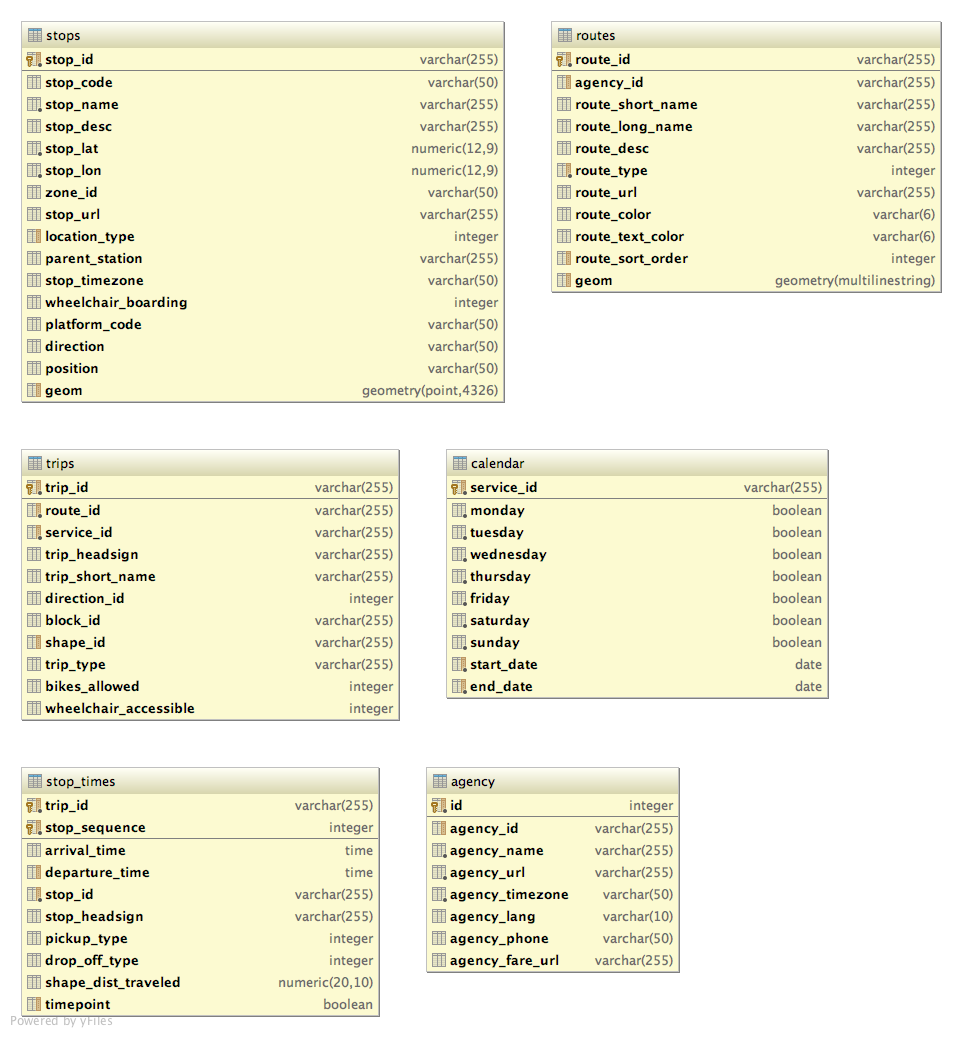
\includegraphics[width=1\textwidth]{gfx/gtfs_uml.png}}
   \caption{Felder innerhalb von GTFS Daten}
   \label{fig:gtfs_uml}
\end{figure}

\section{Levenshtein Distanz zur Ermittlung der Ähnlichkeit zweier Bahnhofsnamen}
\label{sec:appendix:levenshtein}
Die \textit{Levenshtein Distanz} zwischen zwei Zeichenketten gibt die Anzahl der Editieroperationen zurück, die notwendig sind um die eine Zeichenkette in die andere zu transformieren.
Der Größe des ermittelten Wertes kann, je nach Länge der Zeichenketten variieren. 
Die verwendete Bibliothek \textit{java-string-similarity}\footnote{https://github.com/tdebatty/java-string-similarity} bietet die Möglichkeit, eine normalisierte Levenshtein-Distanz zu ermitteln. Dazu wird die ermittelte Levenshtein-Distanz anschließend durch die Länge der längsten Zeichenkette dividiert.
Diese Operation ergibt ein Interval $[0,1]$.

Nun musste ein Algorithmus entwickelt werden, der die normalisierte Levenshtein-Distanz ein bisschen besser auf das Themengebiet Bahnhofsbezeichnungen vorbereitet. Ein Beispiel hierfür sind die Zeichenketten \texttt{''Hauptbahnhof Berlin''} und \texttt{''Berlin Hauptbahnhof''}. Offensichtlich bezeichnen diese den selben Bahnhof, jedoch entspricht die Levenshtein-Distanz zwischen den Zeichenketten $14$ und die normalisierte Levenshtein-Distanz $14/19\approx0,737$.
 
Ich entschied mich dazu, die Zeichenketten vor dem Vergleich zu \textit{tokenizen}, das bedeutet die Zeichenkette anhand bestimmter Trennungszeichen in eine Liste aus Teilzeichenketten aufzuteilen. Dazu wurde die Klasse \texttt{java.util.StringTokenizer} verwendet (Siehe Listing \ref{lev_sum} Zeile 74-81). Anschließend werden die Tokens der beiden zu vergleichenden Zeichenketten alle miteinander verglichen und die jeweils niedrigsten Levenshtein-Distanzen, gewichtet anhand der Länge des kürzeren Tokens aufsummiert (Siehe Listing \ref{lev_sum}). Dies sorgt zum Beispiel dafür, dass die zu Beginn erwähnten Zeichenketten \texttt{''Hauptbahnhof Berlin''} und \texttt{''Berlin Hauptbahnhof''} eine Distanz von $0$ aufweisen.

\lstset{
  language=Java,
  numbers=left,
  caption=Klasse StringDistance zur Ermittlung der Gleichheit zweier Bahnhofsnamen,
  label=lev_sum,
  keywordstyle=\color{javapurple}\bfseries,
  stringstyle=\color{javared},
  commentstyle=\color{javagreen},
  morecomment=[s][\color{javadocblue}]{/**}{*/},
}
\begin{lstlisting}
package utils;

import com.google.common.collect.HashBasedTable;
import com.google.common.collect.Table;
import info.debatty.java.stringsimilarity.NormalizedLevenshtein;
import info.debatty.java.stringsimilarity.interfaces.NormalizedStringDistance;

import java.util.ArrayList;
import java.util.List;
import java.util.StringTokenizer;

/**
 * Created by Tom Oberhauser
 * Methods for String comparison
 */
public class StringDistance {
  /**
   * Compares two Strings. It returns a weighted sum of the best matching tokens.
   * (eg. "Berlin Hauptbahnhof" and "(Hauptbahnhof) Berlin" would have a distance of 0)
   *
   * @param s1 left String
   * @param s2 right String
   * @return likelihood [0;1] where 0 is equal and 1 is different
   */
  public static double minDistance(final String s1, final String s2) {
    double retVal = 0;
    int n = 0;
    List<String> words_left = tokenize(s1);
    List<String> words_right = tokenize(s2);
    Table<String, String, Double> matcherTable = HashBasedTable.create();
    /*
    compare every left with every right word and fill matcher tables
     */
    for (String wordLeft : words_left) {
      for (String wordRight : words_right) {
        double lev = levenshtein(wordLeft, wordRight);
        matcherTable.put(wordLeft, wordRight, lev);
      }
    }
    /*
    find smallest values and remove corresponding rows and cols until the table is empty
     */
    while (!matcherTable.isEmpty()) {
      String minRow = null;
      String minCol = null;
      Double minVal = Double.MAX_VALUE;
      for (String row : matcherTable.rowKeySet()) {
        for (String col : matcherTable.columnKeySet()) {
          Double currentCell = matcherTable.get(row, col);
          if (currentCell < minVal) {
            minRow = row;
            minCol = col;
            minVal = currentCell;
          }
        }
      }
      if (minRow != null && minCol != null) {
        int minLength = (minRow.length() <= minCol.length()) ? minRow.length() : minCol.length();
        n += minLength;
        retVal += (minVal * (double) minLength);
        matcherTable.row(minRow).clear();
        matcherTable.column(minCol).clear();
      }
    }
    return retVal / n;
  }

  /**
   * Tokenizes a String
   *
   * @param s String
   * @return List of tokens without delimiters
   */
  private static List<String> tokenize(final String s) {
    List<String> list = new ArrayList<>();
    StringTokenizer tokenizer = new StringTokenizer(s, "()[].-,; ", false);
    while (tokenizer.hasMoreTokens()) {
      list.add(tokenizer.nextToken());
    }
    return list;
  }

  /**
   * Calculates the normalized levenshtein distance of two Strings
   *
   * @param s1 left String
   * @param s2 right String
   * @return likelihood [0;1] where 0 is equal and 1 is different
   */
  private static double levenshtein(final String s1, final String s2) {
    NormalizedStringDistance nlv = new NormalizedLevenshtein();
    return nlv.distance(s1, s2);
  }
}
\end{lstlisting}

\section{Kennzahlen zur qualitativen Bewertung eines binären Klassifikators}
\label{sec:appenix:fmeasure}

Ein Klassifikator soll etwas bestimmtes aus gegebenen Merkmalen vorhersagen.
Genauergesagt entspricht ein Klassifikator einer Abbildung eines Merkmalsraumes auf eine Menge von Klassen.
Um Die Qualität dieser Vorhersage bzw. Abbildung zu bewerten, existieren Kennzahlen.
Im folgenden wird auf die Kennzahlen \textit{Precision (Genauigkeit)}, \textit{Recall (Trefferquote)} und \textit{F-Maß} zur qualitativen Bewertung eines binären Klassifikators eingegangen.

Zunächst muss ein Datensatz mit bekannten Ergebnissen vorliegen.
Dieser wird auch Gold-Standard genannt.
Anhand des Gold-Standards können nun Vorhersagen mit bekannten Ergebnissen durchgeführt, und eine \textit{Wahrheitsmatrix} befüllt werden. In Tabelle \ref{tab:wahrheitsmatrix} ist eine Wahrheitsmatrix für die Beispielklassen \texttt{+} und \texttt{-} abgebildet. 
\begin{table}[]
\centering
\caption{Wahrheitsmatrix}
\label{tab:wahrheitsmatrix}
\begin{tabular}{|l|l|l|}
\hline
\textbf{}           & \textbf{Vorhersage +} & \textbf{Vorhersage -} \\ \hline
\textbf{Wahrheit +} & True Positive ($TP$)    & False Negative ($FN$)   \\ \hline
\textbf{Wahrheit -} & False Positive ($FP$)   & True Negative ($TN$)    \\ \hline
\end{tabular}
\end{table}

Anhand der Messwerte $TP, FP, FN, TN$ lassen sich nun Kennzahlen errechnen.

\subsubsection{Precision (Genauigkeit)}

Der \textit{Precision-Wert} gibt das Verhältnis zwischen allen positiven Vorhersagen und den korrekten positiven Vorhersagen an. Vereinfacht gesagt, wie viele von den positiv vorhergesagten Ergebnissen waren korrekt.

$$Precision = \frac{TP}{TP + FP}$$

\subsubsection{Recall (Trefferquote)}

Der \textit{Recall-Wert} gibt das Verhältnis zwischen allen korrekt als positiv vorhergesagten Objekte an der Gesamtheit der tatsächlich positiven Objekte an. Vereinfacht gesagt, wie viele positive Ergebnisse wurden wirklich gefunden.
$$Recall = \frac{TP}{TP + FN}$$

\subsubsection{F-Maß}

Die Kennzahlen \textit{Precision} und \textit{Recall} alleine ergeben noch keine gute Abbildung der Vorhersagequalität.
Beispielsweise lässt sich der Precision-Wert anheben, in dem der Klassifikator nur ein einzelnes Ergebnis als \texttt{+} korrekt klassifiziert.
Alle als \texttt{+} vorhergesagten Werte währen dann in diesem Fall korrekt.
Aus diesem Grund gibt es das \textit{F-Maß}, welche beide Werte miteinander vereint und als Qualitätskriterium verwendet werden kann.

$$F = 2 * \frac{Precision * Recall}{Precision + Recall}$$
\cleardoublepage

% --------------------------
% Back matter
% --------------------------
{%
\setstretch{1.1}
\renewcommand{\bibfont}{\normalfont\small}
\setlength{\biblabelsep}{0pt}
\setlength{\bibitemsep}{0.5\baselineskip plus 0.5\baselineskip}
\printbibliography[nottype=online]
\printbibliography[heading=subbibliography,title={Online-Quellen},type=online,prefixnumbers={@}]
}
\cleardoublepage

%\listoffigures
%\cleardoublepage
%\listoftables
%\cleardoublepage

% !TEX root = ../thesis-example.tex
%
%************************************************
% Declaration
%************************************************
\pdfbookmark[0]{Declaration}{Declaration}
\chapter*{Declaration}
\label{sec:declaration}
\thispagestyle{empty}

You can put your declaration here, to declare that you have completed your work solely and only with the help of the references you mentioned.

\bigskip

\noindent\textit{\thesisUniversityCity, \thesisDate}

\smallskip

\begin{flushright}
	\begin{minipage}{5cm}
		\rule{\textwidth}{1pt}
		\centering\thesisName
	\end{minipage}
\end{flushright}

%*****************************************
%*****************************************

%\clearpage
%\newpage
\mbox{}

% **************************************************
% End of Document CONTENT
% **************************************************
\end{document}
